
The code is composed of different parts working together, and when problems occur, it is important to identify their source in order to correct them. \\
The main issues are:

\begin{itemize}
    \setlength\itemsep{0pt}
    \setlength\parskip{0pt}
    \item \textbf{Logic code errors}
    \item \textbf{Errors in matrix data storage}
    \item \textbf{Inference computation errors}
\end{itemize}

\noindent
Different techniques were used to debug the system, as explained below.

\subsection{Debug print methodology}

To debug the code, the JTAG-UART peripheral was used to print debug messages. \\
However, UART messages must be written into a buffer, and if too many messages are generated, the buffer can become full, resulting in code slowdown and an excessive amount of printed output. \\
To avoid this problem, conditional compilation was used to define a \\\texttt{DEBUG\_PRINTF()} macro that prints data through the UART only if the constant \texttt{DEBUG} is defined; otherwise, the macro does nothing. \\
An example of this implementation is shown in \autoref{lst:debug_print()}, where \texttt{printf()} is the standard C function defined in the \texttt{stdio.h} library that prints data through the UART, and \texttt{matrix\_print()} is a function defined in the \texttt{matrix\_lib.h} library that internally uses the \texttt{printf()} function to print the data contained in a \texttt{Matrix} structure. The \texttt{Matrix} type is defined in \texttt{matrix\_lib.h} and described in \autoref{sssec:matrix_library}.

\vspace{1em}
\begin{lstlisting}[language=C, caption={\texttt{DEBUG\_PRINT()} macro definition for the NN library}, label={lst:debug_print()}, morekeywords={Matrix,\#include,\#define,\#ifdef,\#ifndef,\#else,\#endif}, alsoletter={\#}]
    #include <stdio.h>
    #include "matrix_lib.h"
    
    // Comment this line to disable debugging messages
    #define NN_LIB_DEBUG
    
    #ifdef NN_LIB_DEBUG
        #define DEBUG_NN_PRINTF(...)    printf(__VA_ARGS__)
        #define DEBUG_NN_MATRIX_PRINTF(m)   matrix_print(m)
    #else 
        #define DEBUG_NN_PRINTF(...)
        #define DEBUG_NN_MATRIX_PRINTF(m)
    #endif
\end{lstlisting}

\newpage
\subsubsection{Python Matrix visualization}

The letters shown on the LCD are stored in a \(140 \times 140\) matrix. \\
Each element of the matrix contains the value \(1.0\) if the corresponding pixel is colored, and \(0.0\) otherwise. \\
The matrix is then resized to a smaller \(28 \times 28\) version. \\
To verify that the resizing and processing steps work correctly, a debug print was used to display the matrix values, together with a Python script that visualizes the generated data. \\
In \autoref{fig:emnist_char_confrot}, a comparison between a letter written on the LCD and a letter taken from the dataset is shown.

\begin{figure}[h!]
    \centering
    
\includegraphics[width=0.65\linewidth]{img/emnist_char_confrot.jpg}
    \caption{On the left is shown a letter "a" from the dataset, while on the right is shown a letter "a" written manually on the screen}
    \label{fig:emnist_char_confrot}
\end{figure}

\subsection{Python Neural Network confront}

The last aspect to verify is the inference computation of the neural network. \\
To do this, the same network was implemented in Python using the PyTorch library. \\
The weights and biases were then loaded into the network. \\
After that, several inputs were processed using both the Python implementation and the network programmed into the FPGA, and the corresponding output values were compared to verify that they match. \\
In \autoref{tab:comparison_results}, we can see the maximum output error obtained when recognizing the letter "a" shown in \autoref{fig:emnist_char_confrot}.

\begin{table}[h!]
    \centering
    \begin{tabular}{l c}
    
        \hline
        Metric & Value \\
        \hline
        Predicted class & 36 \\
        Corresponding character & "a" \\
        Max absolute error & \(3.8147 \cdot 10^{-6}\) \\
        \hline
        
    \end{tabular}
    \caption{Comparison between FPGA and PyTorch inference outputs}
    \label{tab:comparison_results}
\end{table}

\subsection{Neural Network accuracy}
\label{sssec:nn_accuracy_tst}

The neural network training was performed in Python using a library called PyTorch. \\
Using this library, the neural network was instantiated layer by layer, and the activation functions were also defined. \\
To perform different tests, two fully connected neural networks with three layers were defined, making them easier to implement using the Neural Network library developed in C for the Nios II processor. \\
One network was trained to recognize only numbers, while the other was trained to recognize both letters and numbers. \\
The datasets used were the MNIST dataset for digit recognition and the EMNIST dataset for alphanumeric character recognition. \\
The code used to instantiate the network in python is shown in \autoref{lst:NN_python_def}.

\vspace{1em}
\begin{lstlisting}[language=python, caption={MNIST letter recognition neural network definition in python using PyTorch}, label={lst:NN_python_def}]
    class Net(nn.Module):
        def __init__(self):
            super(Net, self).__init__()
            #input matrix 28x28 flattened
            self.fc1 = nn.Linear(784, 256)
            #hidden layer with 256 inputs and 128 outputs
            self.fc2 = nn.Linear(256, 128)
            #output vector of 10 numbers
            self.fc3 = nn.Linear(128, 10)
    
        # x represents our data
        def forward(self, x):
            #flattening the 28x28 input matrix
            x = torch.flatten(x, 1)
            #computing the output matrix
            x = F.relu(self.fc1(x))
            x = F.relu(self.fc2(x))
            x = self.fc3(x) 
            #return the output matrix
            return x
\end{lstlisting}

\noindent
With the same method has been defined also the network for EMNIST dataset (for letters and numbers). \\
The training has been done with a minibatch of \(256\) elements taken randomly from the dataset; this means that weights and biases of the network are updated using a subset of the dataset to reduce the computational complexity. \\
Every time that the entire minibatch has been sent to the network and the weights and biases updated, a training epoch is completed. \\
Every epoch of training, the program do a test with \(2000\) elements taken randomly from the dataset and test the accuracy of the network and the average training loss. \\
The accuracy (\(Acc\)) is defined as the number of correct guess of the network over the total, and the average loss (\(\mathcal{L}_{\text{avg}}\)) is defined as the average difference of the computed output from the ideal output (\autoref{eq:NN_metrics_calc}).

\begin{equation}
    \begin{aligned}
        \text{Acc} &= \frac{N_{\text{correct}}}{N} \\
        \mathcal{L}_{\text{avg}} &= \frac{1}{N} \sum_{i=1}^{N} \left\| \vec{a}_i - \vec{y}_i \right\|
    \end{aligned}
    \label{eq:NN_metrics_calc}
\end{equation}

\noindent
where:

\begin{itemize}
    \setlength\itemsep{0pt}
    \setlength\parskip{0pt}
    \item \(N\): total number of samples
    \item \(N_{\text{correct}}\): number of correctly predicted samples
    \item \(\vec{a}_i\): computed output for sample \(i\)
    \item \(\vec{y}_i\): predicted output for sample \(i\)
\end{itemize}

\noindent
A graph of accuracy and training loss during a \(30\)-epoch training was produced for both models (MNIST and EMNIST), as shown in \autoref{fig:graph_metrics}.

\begin{figure}[h!]
    \centering
    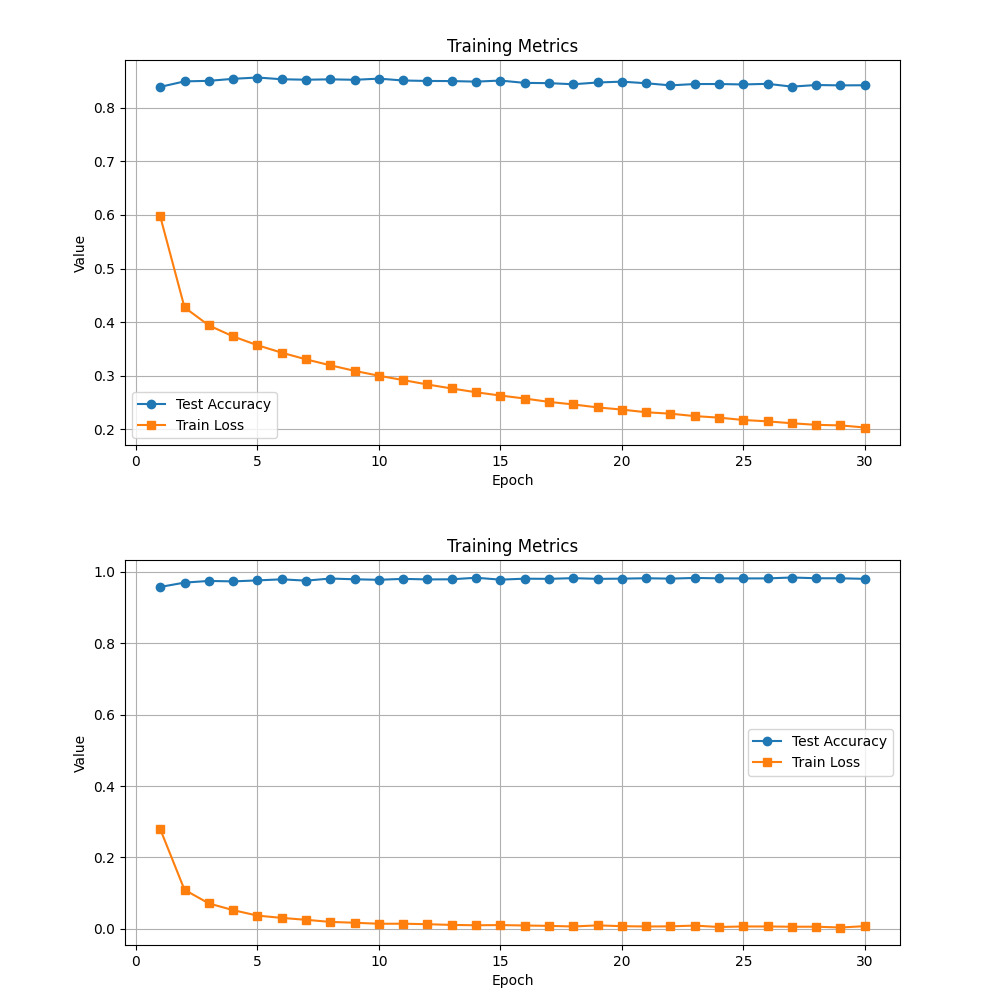
\includegraphics[width=0.8\linewidth]{img/metrics_graph_EMNIST_up.jpg}
    \caption{Metrics graph: the bottom graph shows the MNIST dataset, while the upper graph shows the EMNIST dataset}
    \label{fig:graph_metrics}
\end{figure}

\noindent
As can be seen from \autoref{fig:graph_metrics}, for both networks the accuracy saturates after approximately \(5\) epochs. \\
However, for the MNIST dataset, the test accuracy also saturates after approximately \(10\) epochs, whereas for the EMNIST dataset the test accuracy saturates after approximately \(30\) epochs. \\
The weights and biases matrix used for inference inside the niosII has been generated after \(30\) epochs of training for both datasets.

\vspace{3em}
\noindent
\textit{Note: Even if the accuracy for the EMNIST dataset is approximately \(85\%\), the dataset contains letters that occupy the entire \(28 \times 28\) matrix, while on the LCD writing area (after downscaling) the letters usually occupy a smaller region. \\
For this reason, the training was performed by reducing the size of the dataset letters. \\
This effect can also be seen in \autoref{fig:emnist_char_confrot} where the letter from the dataset is bigger than the one written manually on the screen.}

\subsection{Neural Network inference time}
\label{sssec:nn_inf_time}

Once the neural network had been implemented on the FPGA, two operations were performed to improve the inference time.

\begin{itemize}
    \setlength\itemsep{0pt}
    \setlength\parskip{0pt}
    \item A hardware floating-point operator was instantiated to accelerate, through hardware, the mathematical operations involving weights and biases, \\
    mainly additions and multiplications.
    \item The compiler optimization settings were enabled to optimize the generated code (optimization level 3).
\end{itemize}

\noindent
To evaluate the improvement introduced by each modification to the inference time, the inference execution time was measured via software, and the average inference time was analyzed both with and without these optimizations.

\begin{table}[h!]
    \centering
    \begin{tabular}{l c}
    
        \hline
        Optimization & Inference time \\
        \hline
        No hardware fp. operator, No compiler optimization   & \(6.101 \; s\) \\
        No hardware fp. operator, With compiler optimization & \(3.150 \; s\) \\
        With hardware fp. operator, No compiler optimization & \(2.089 \; s\) \\
        With hardware fp. operator and Compiler optimization & \(0.509 \; s\) \\
        \hline
        
    \end{tabular}
    \caption{Inference Time Dependence on Optimization Methods}
    \label{tab:inf_time_confront}
\end{table}

\newpage
\subsection{Project Demonstration}
\label{sssec:project_demo}

The following images show the user drawing a character on the screen and the neural network recognizing the character drawn, then showing it in the letter box area on the top section of the screen. 

\begin{figure}[h!]
    \centering
    \begin{subfigure}[t]{0.45\textwidth}
        \centering
        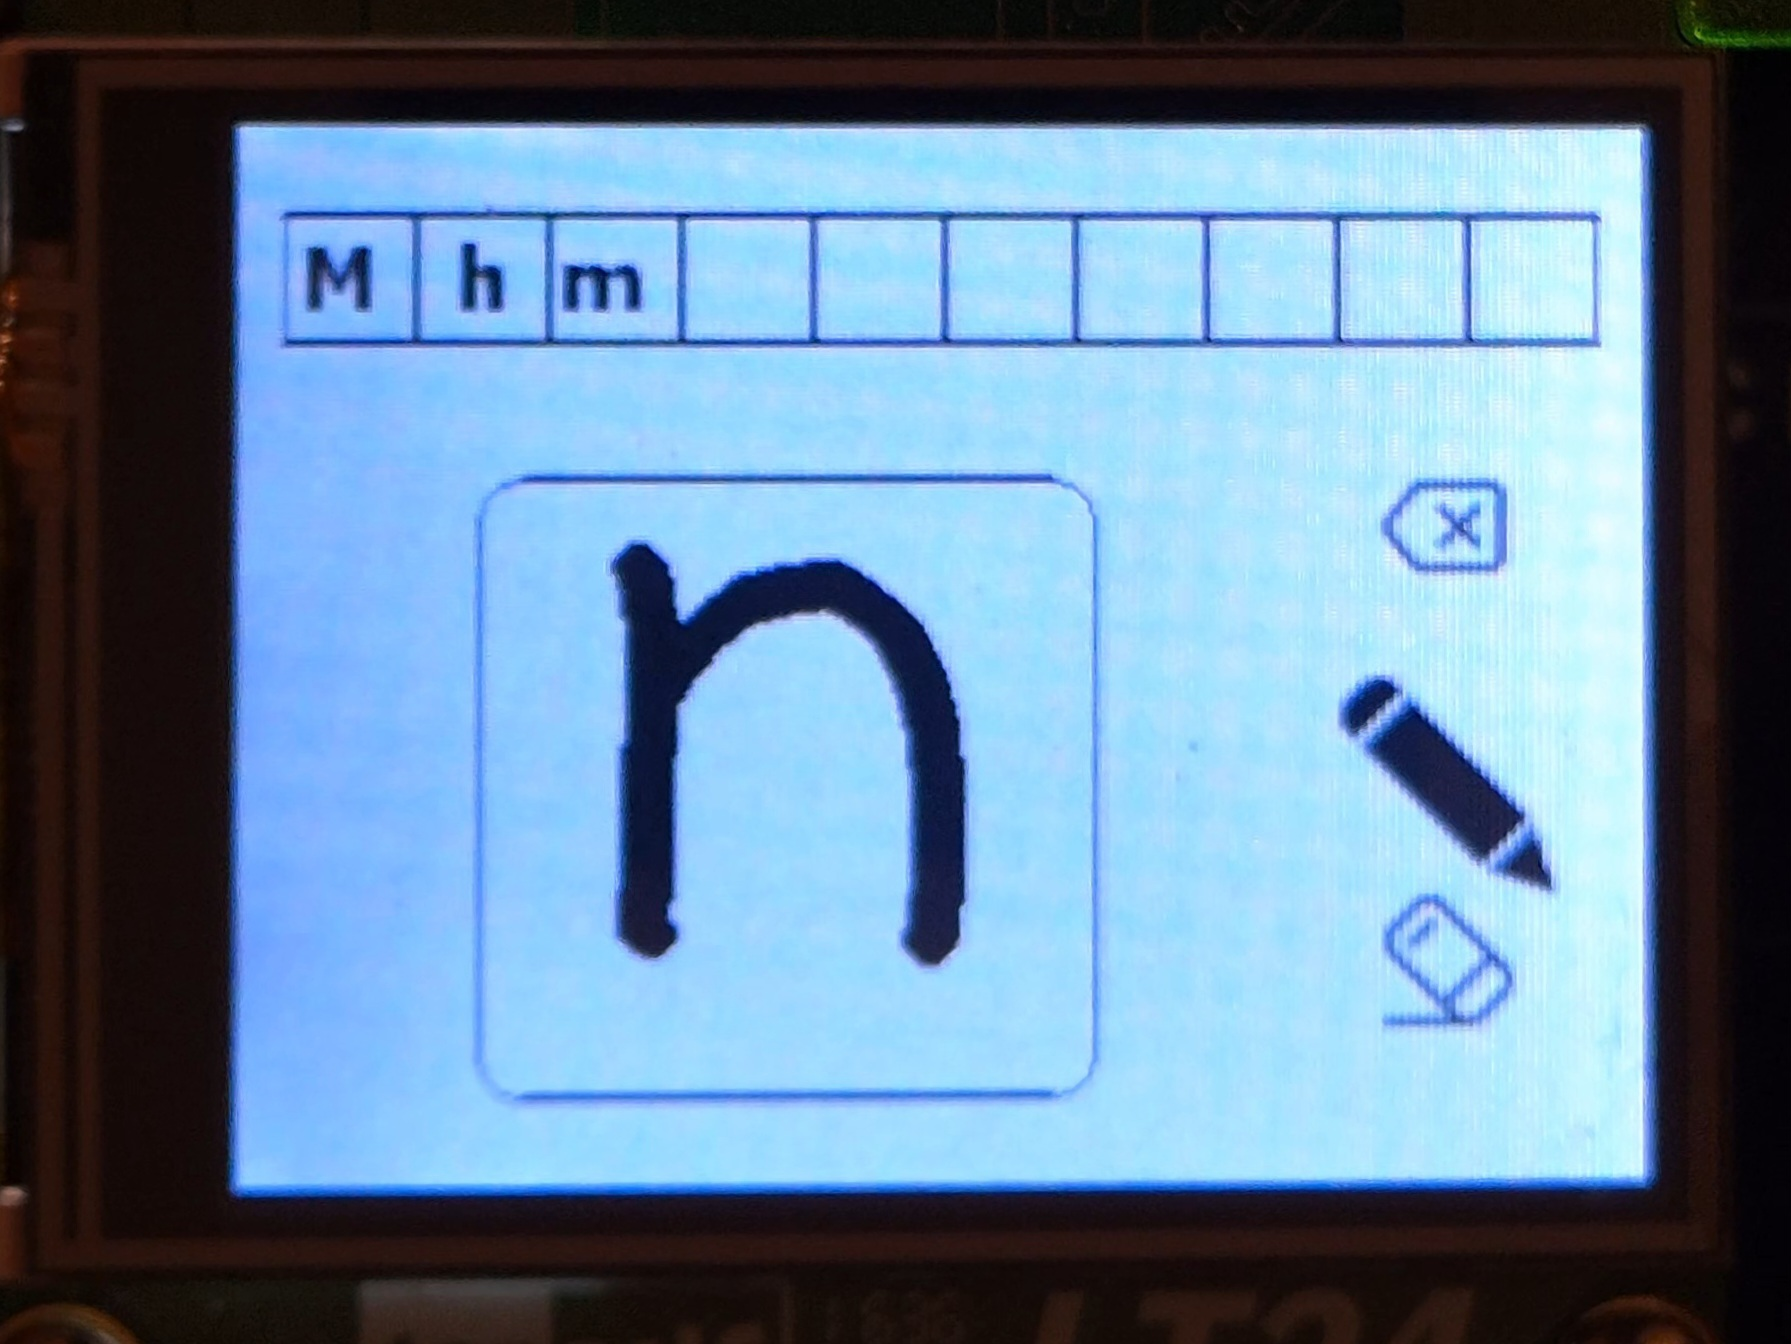
\includegraphics[width=\textwidth, height=3.5cm, keepaspectratio=false]{img/n_drawing.jpg} 
        \caption{Letter "n" drawn by the user}
        \label{fig:sub1}
    \end{subfigure}
    \hfill 
    \begin{subfigure}[t]{0.45\textwidth}
        \centering
        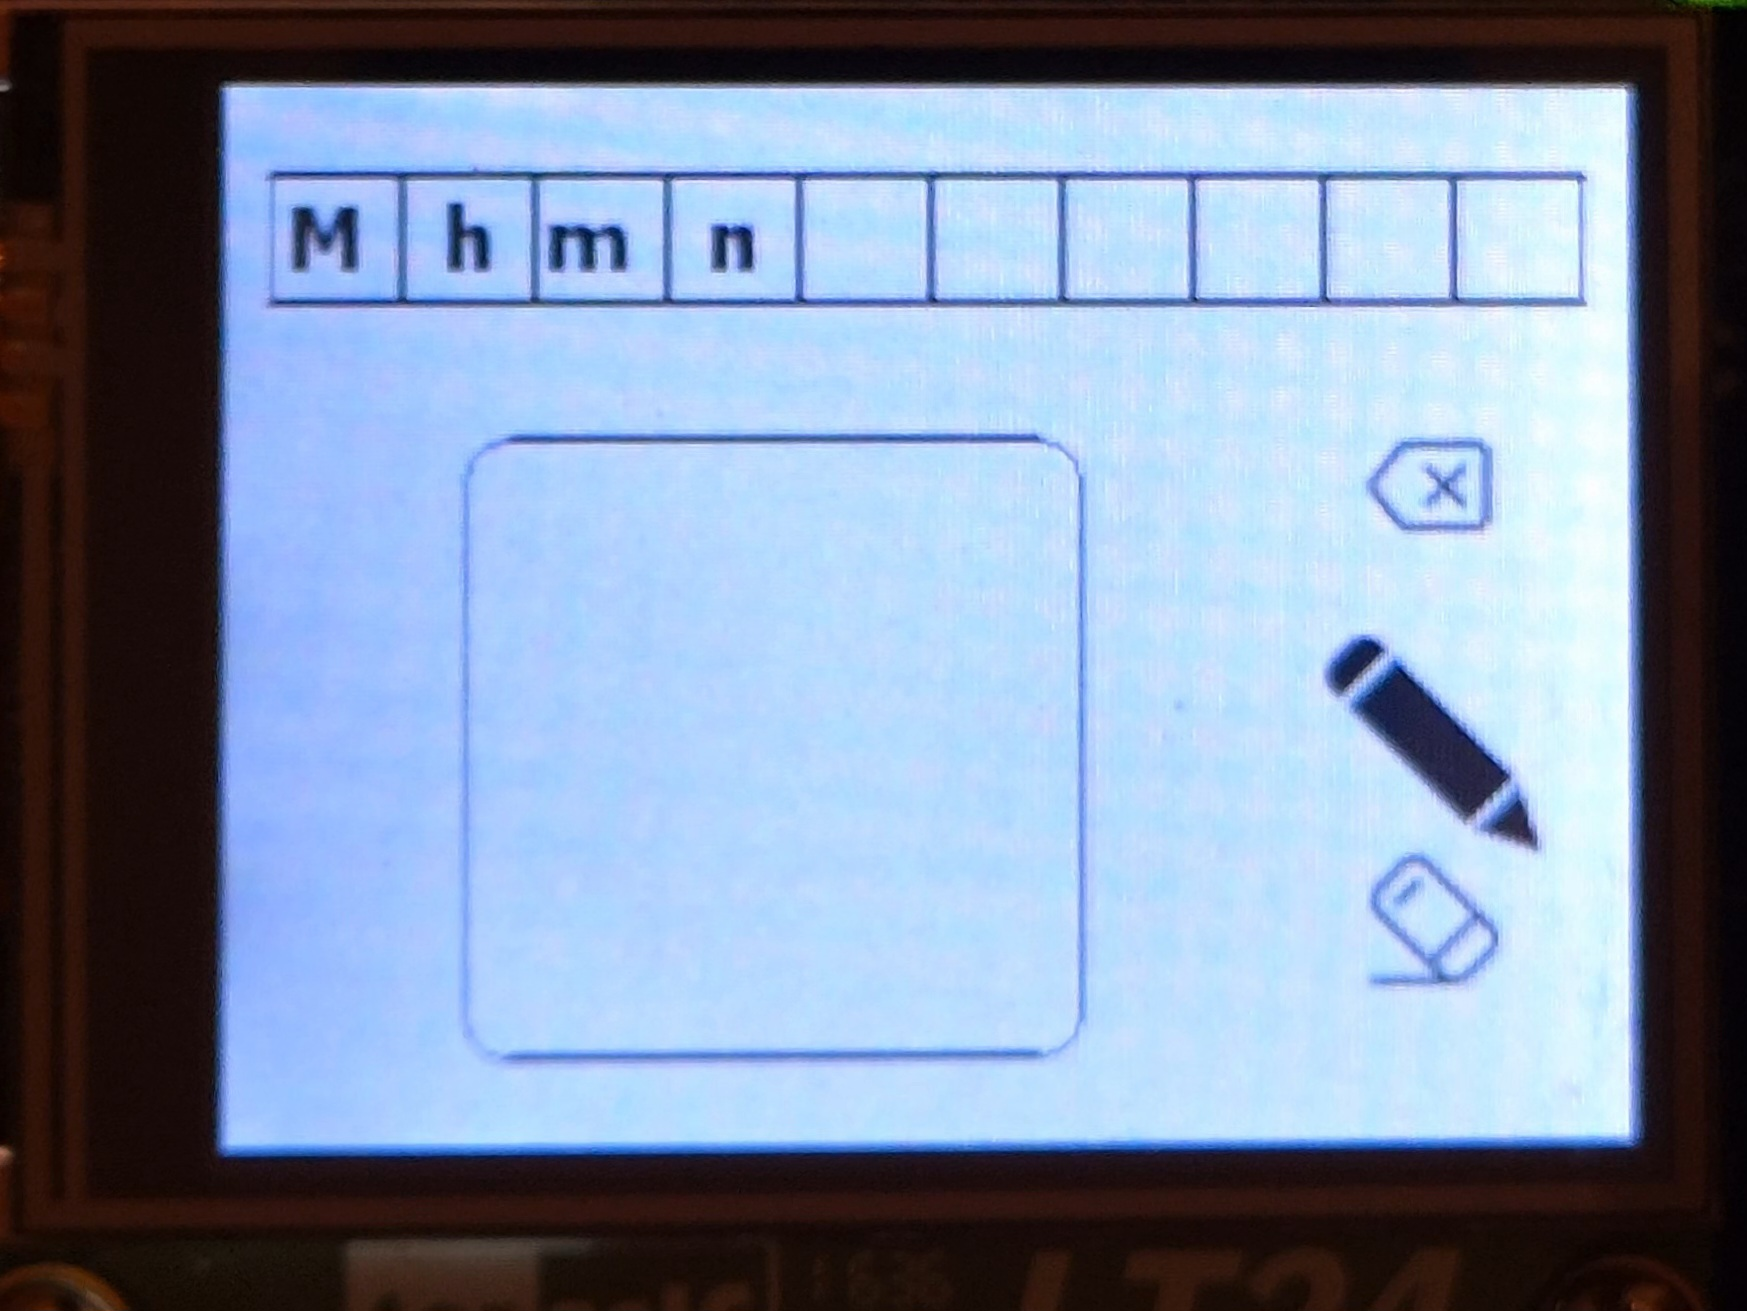
\includegraphics[width=\textwidth, height=3.5cm, keepaspectratio=false]{img/n_letterbox.jpg} 
        \caption{Letter "n" recognized by the NN}
        \label{fig:sub2}
    \end{subfigure}
    
    \caption{Showcasing the recognition of the letter "n"}
    \label{fig:letter_n}
\end{figure}

\begin{figure}[h!]
    \centering
    \begin{subfigure}[t]{0.45\textwidth}
        \centering
        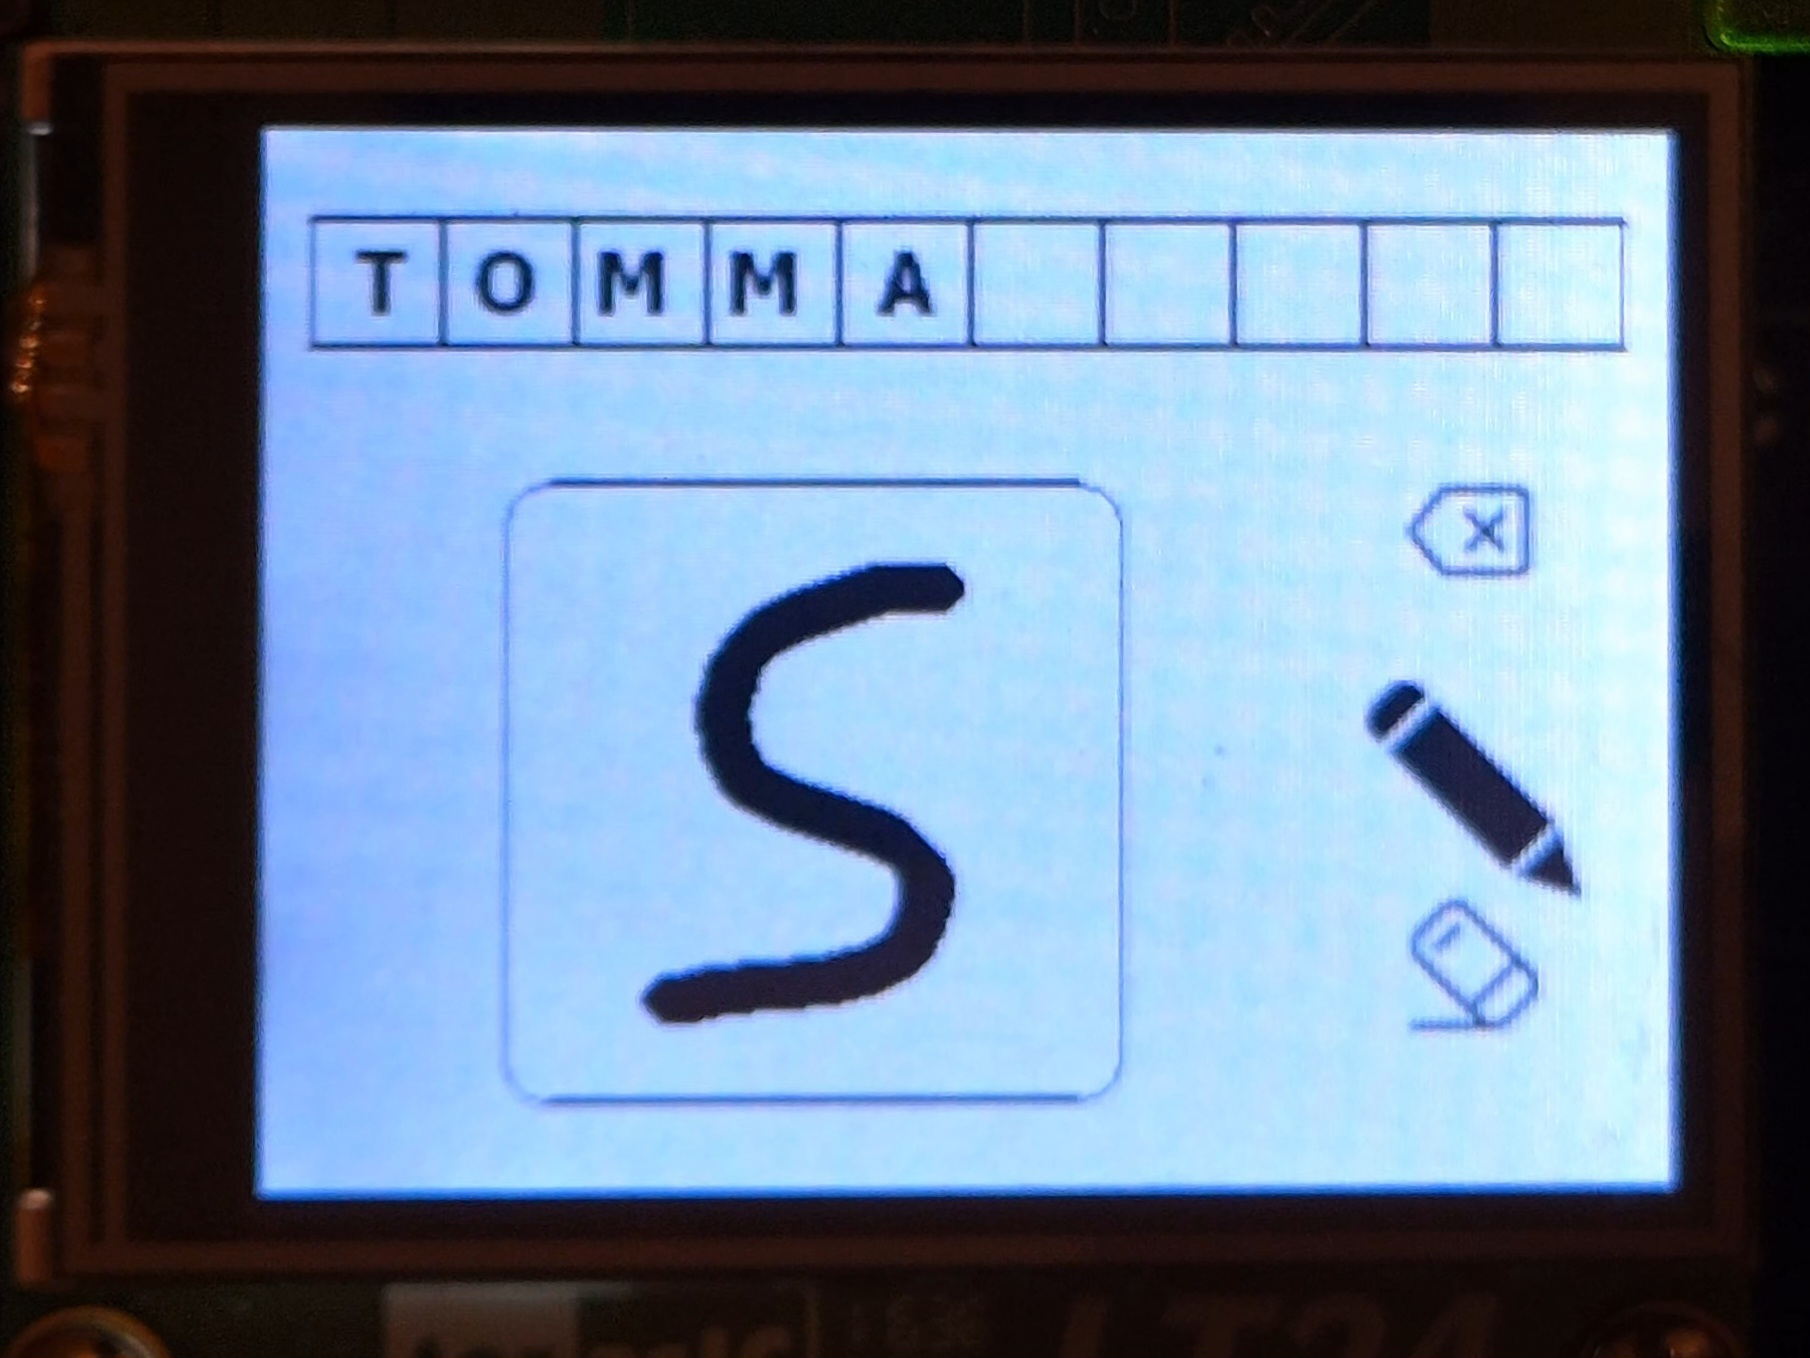
\includegraphics[width=\textwidth, height=3.5cm, keepaspectratio=false]{img/S_drawing.jpg} 
        \caption{Letter "S" drawn by the user}
        \label{fig:sub3}
    \end{subfigure}
    \hfill 
    \begin{subfigure}[t]{0.45\textwidth}
        \centering
        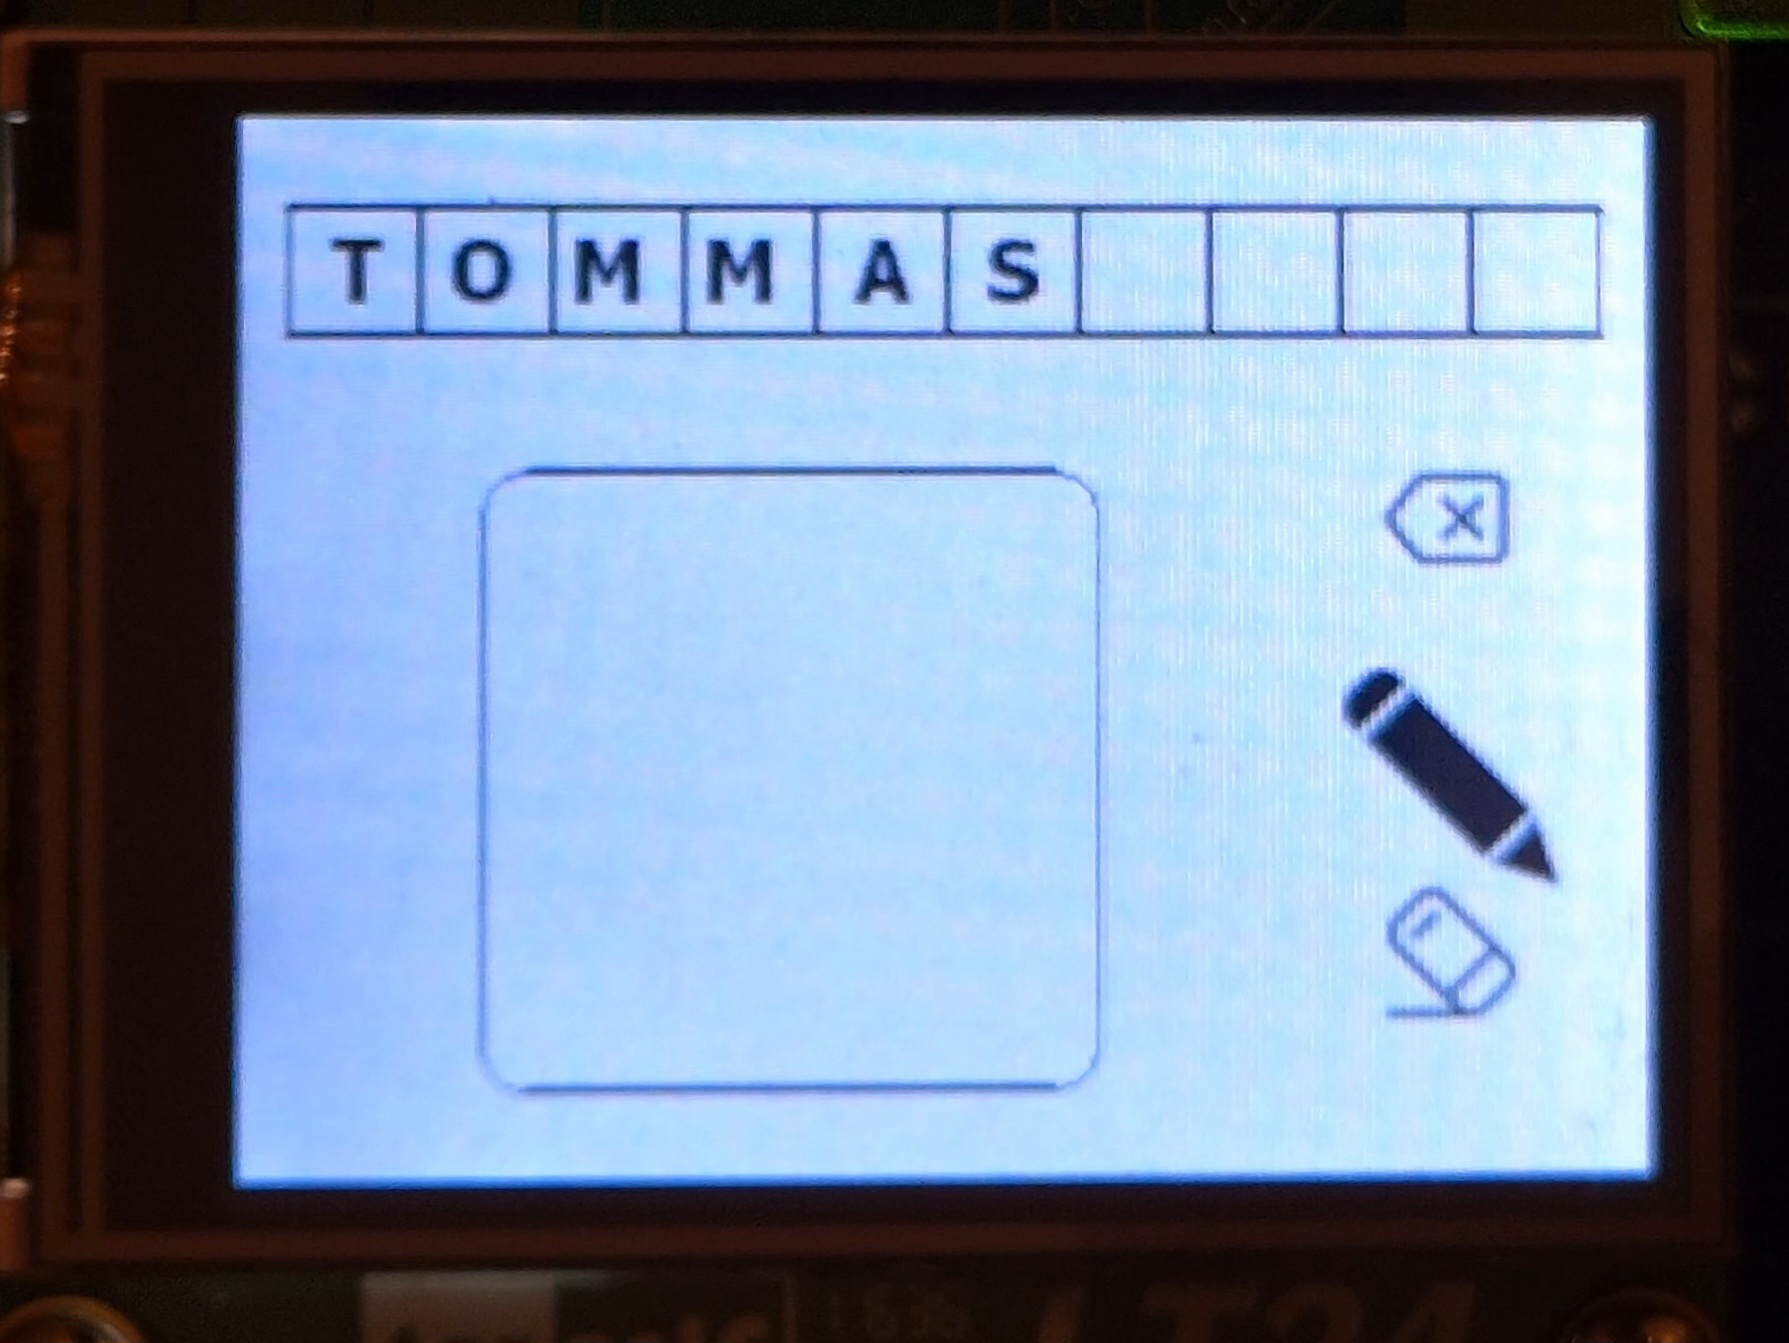
\includegraphics[width=\textwidth, height=3.5cm, keepaspectratio=false]{img/S_letterbox.jpg} 
        \caption{Letter "S" recognized by the NN}
        \label{fig:sub4}
    \end{subfigure}
    
    \caption{Showcasing the recognition of the letter "S"}
    \label{fig:letter_S}
\end{figure}

\begin{figure}[h!]
    \centering
    \begin{subfigure}[t]{0.45\textwidth}
        \centering
        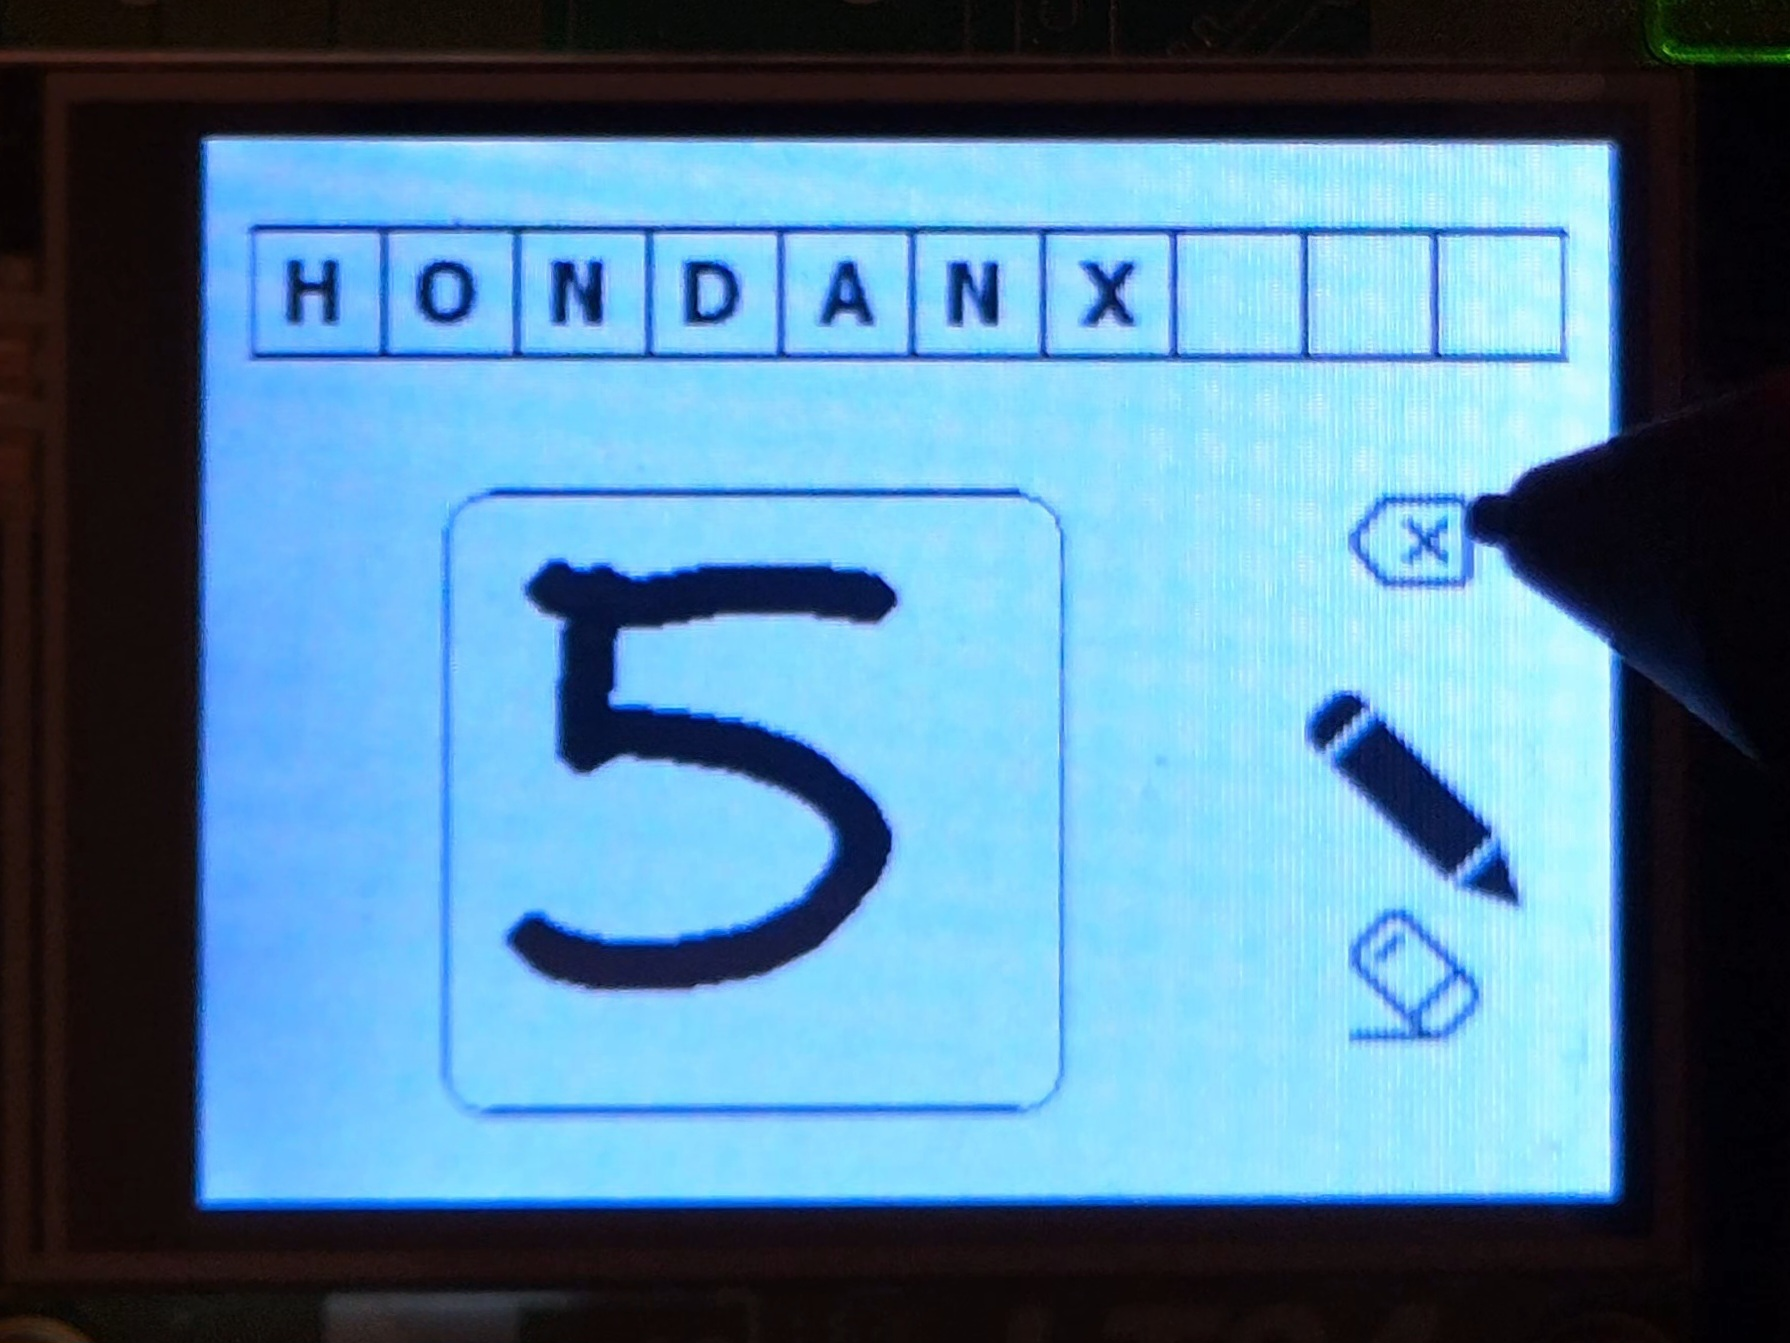
\includegraphics[width=\textwidth, height=3.5cm, keepaspectratio=false]{img/5_drawing.jpg} 
        \caption{Number "5" drawn by the user}
        \label{fig:sub5}
    \end{subfigure}
    \hfill 
    \begin{subfigure}[t]{0.45\textwidth}
        \centering
        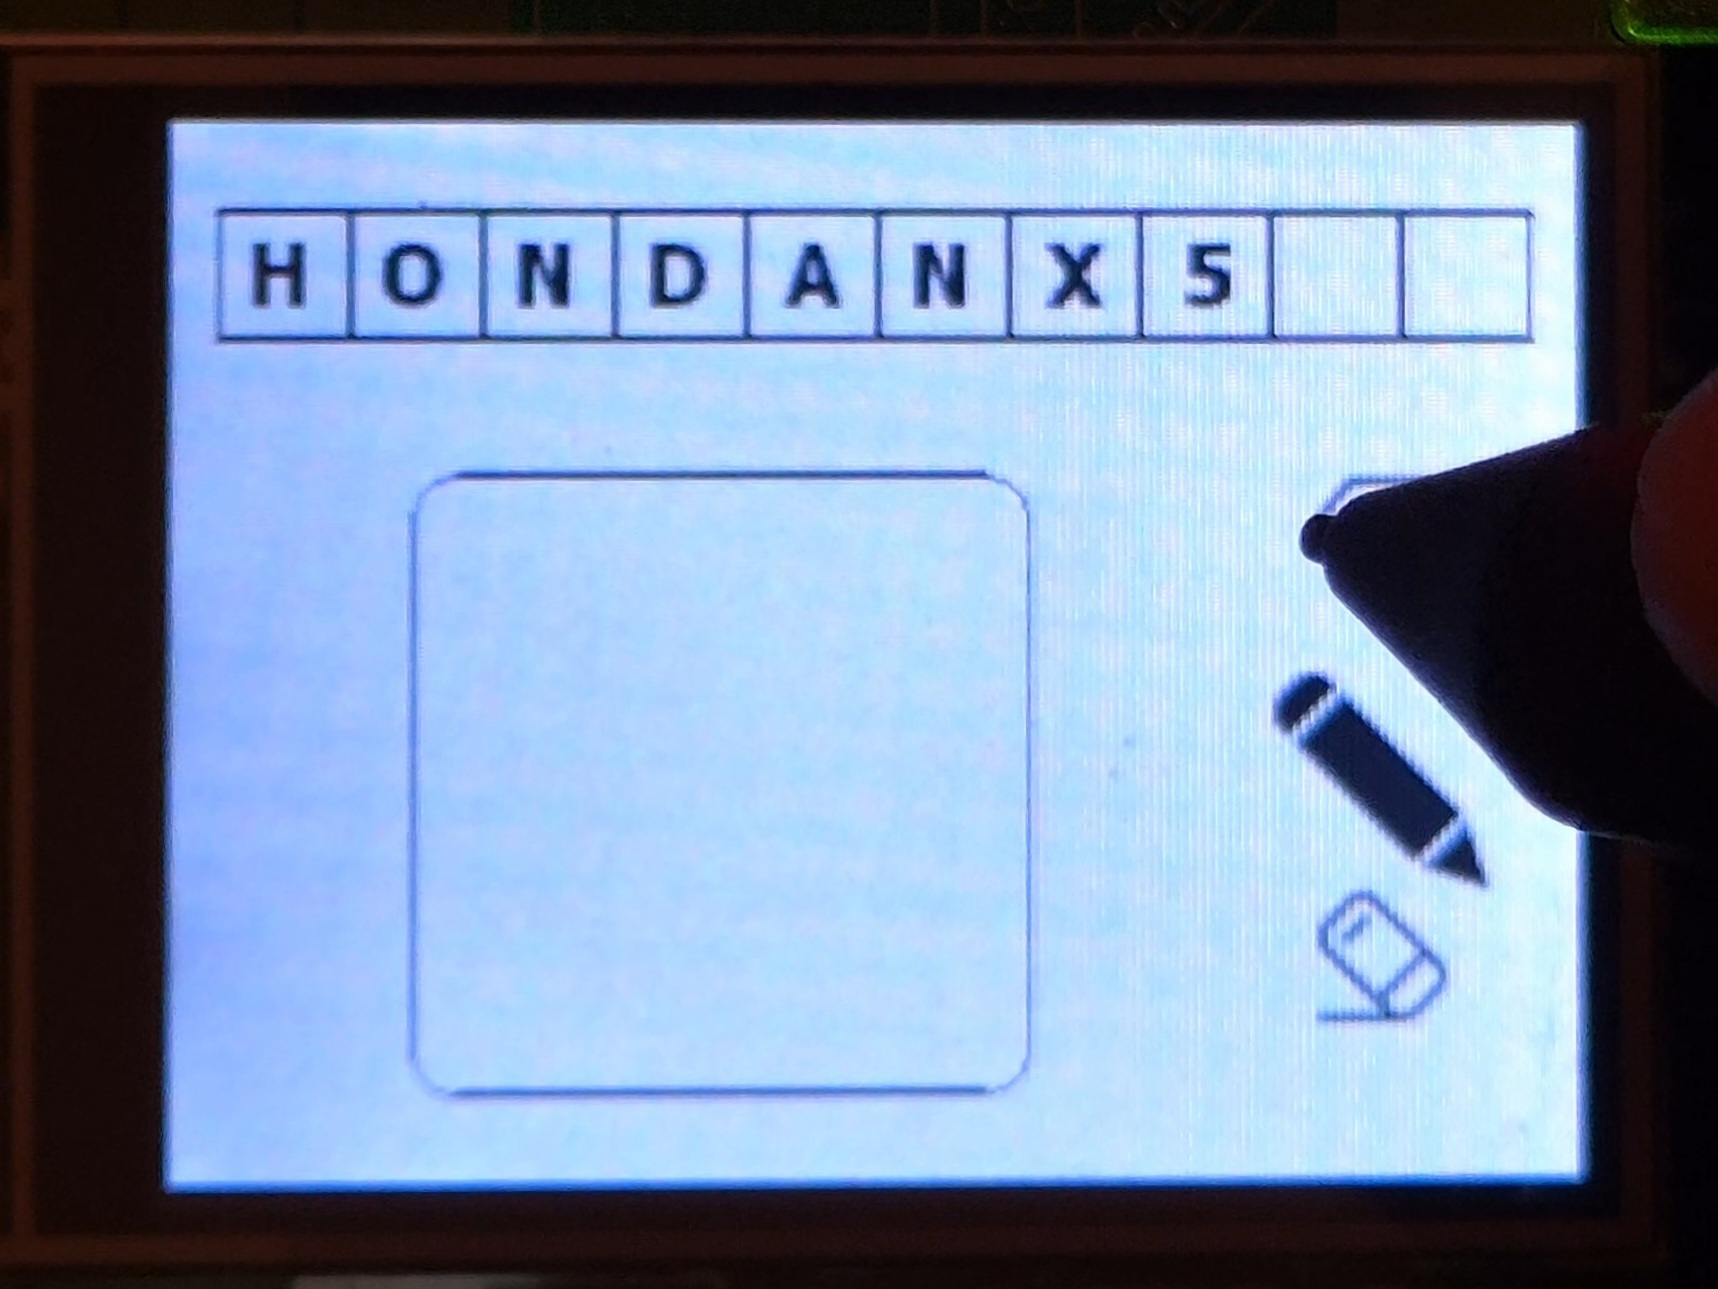
\includegraphics[width=\textwidth, height=3.5cm, keepaspectratio=false]{img/5_letterbox.jpg} 
        \caption{Number "5" recognized by the NN}
        \label{fig:sub6}
    \end{subfigure}
    
    \caption{Showcasing the recognition of the number "5"}
    \label{fig:number_5}
\end{figure}

\newpage